\documentclass[conference]{IEEEtran}
%% SECON 2013 addition:
\makeatletter
\def\ps@headings{%
\def\@oddhead{\mbox{}\scriptsize\rightmark \hfil \thepage}%
\def\@evenhead{\scriptsize\thepage \hfil \leftmark\mbox{}}%
\def\@oddfoot{}%
\def\@evenfoot{}}
\makeatother
\pagestyle{headings} 

\ifCLASSINFOpdf
  % \usepackage[pdftex]{graphicx}
  % declare the path(s) where your graphic files are
  % \graphicspath{{../pdf/}{../jpeg/}}
  % and their extensions so you won't have to specify these with
  % every instance of \includegraphics
  % \DeclareGraphicsExtensions{.pdf,.jpeg,.png}
\else
  % or other class option (dvipsone, dvipdf, if not using dvips). graphicx
  % will default to the driver specified in the system graphics.cfg if no
  % driver is specified.
  % \usepackage[dvips]{graphicx}
  % declare the path(s) where your graphic files are
  % \graphicspath{{../eps/}}
  % and their extensions so you won't have to specify these with
  % every instance of \includegraphics
  % \DeclareGraphicsExtensions{.eps}
\fi
% *** MATH PACKAGES ***
%
\usepackage[cmex10]{amsmath}
\usepackage{amsfonts}
\usepackage{graphicx, epsfig}
\usepackage{color}
\usepackage{subfigure}
\usepackage{xspace}
\usepackage{algorithm}
\usepackage{algpseudocode}
\usepackage{breqn}
\usepackage{cite}

\renewcommand{\thealgorithm}{}
\algnewcommand{\LineComment}[1]{\State \(\triangleright\) #1}
% A popular package from the American Mathematical Society that provides
% many useful and powerful commands for dealing with mathematics. If using
% it, be sure to load this package with the cmex10 option to ensure that
% only type 1 fonts will utilized at all point sizes. Without this option,
% it is possible that some math symbols, particularly those within
% footnotes, will be rendered in bitmap form which will result in a
% document that can not be IEEE Xplore compliant!
%
%\usepackage{array}
%\usepackage{mdwmath}
%\usepackage{mdwtab}
%\usepackage{eqparbox}
%\usepackage[tight,footnotesize]{subfigure}
%\usepackage[caption=false]{caption}
%\usepackage[font=footnotesize]{subfig}
%\usepackage[caption=false,font=footnotesize]{subfig}
%
%\usepackage{fixltx2e}

%\usepackage{stfloats}

%\usepackage{url}

% correct bad hyphenation here
\hyphenation{net-works}

\DeclareMathOperator*{\E}{\mathbb{E}}

\begin{document}
%
% paper title
% can use linebreaks \\ within to get better formatting as desired
\title{Simulation Details and Results}

\IEEEoverridecommandlockouts

% author names and affiliations
% use a multiple column layout for up to three different
% affiliations

%\author{\IEEEauthorblockN{Scott Rager}
%\IEEEauthorblockA{Department of Computer Science and Engineering\\
%Pennsylvania State University\\
%University Park, PA 16802\\
%Email: rager@psu.edu}}

%\author{\IEEEauthorblockN{Scott Rager, Ertugrul Ciftcioglu, Thomas La Porta}
%\IEEEauthorblockA{Department of Computer Science\\
%and Engineering\\
%Pennsylvania State University\\
%University Park, PA 16802\\
%Email: rager@psu.edu, enc118@psu.edu, tlp@cse.psu.edu}
%\and
%\IEEEauthorblockN{Alice Leung, William Dron}
%\IEEEauthorblockA{Raytheon BBN Technologies\\
%Cambridge, MA 02138\\
%Email: aleung@bbn.com, wdron@bbn.com}
%\and
%\IEEEauthorblockN{John Hancock}
%\IEEEauthorblockA{Artistech\\
%City, State Zip Code\\
%Email: johnh@artistech.com}
%}

%\author{
%  \IEEEauthorblockN{Scott T. Rager\IEEEauthorrefmark{1} \quad Ertugrul N. Ciftcioglu\IEEEauthorrefmark{1} \quad
%    \quad Thomas F. La Porta\IEEEauthorrefmark{1} \\ Alice Leung\IEEEauthorrefmark{2} \quad William Dron\IEEEauthorrefmark{2} \quad John Hancock\IEEEauthorrefmark{3} \\
%  }
%  \IEEEauthorblockA{
%  	\IEEEauthorrefmark{1}The Pennsylvania State University, University Park, PA 16802\\
%  \IEEEauthorrefmark{2}Raytheon BBN Technologies, Cambridge, MA 02138\\
%  \IEEEauthorrefmark{3}Artistech, Inc., Fairfax, VA 22030
%  }
%
%  Email:  str5004@psu.edu, enc118@psu.edu, tlp@cse.psu.edu, aleung@bbn.com, wdron@bbn.com, johnh@artistech.com
%\thanks{Research was sponsored by the U.S. Army Research Laboratory under the Network Science Collaborative Technology Alliance, Agreement Number W911NF-09-2-0053.} }


% for over three affiliations, or if they all won't fit within the width
% of the page, use this alternative format:
% 
%\author{\IEEEauthorblockN{Michael Shell\IEEEauthorrefmark{1},
%Homer Simpson\IEEEauthorrefmark{2},
%James Kirk\IEEEauthorrefmark{3}, 
%Montgomery Scott\IEEEauthorrefmark{3} and
%Eldon Tyrell\IEEEauthorrefmark{4}}
%\IEEEauthorblockA{\IEEEauthorrefmark{1}School of Electrical and Computer Engineering\\
%Georgia Institute of Technology,
%Atlanta, Georgia 30332--0250\\ Email: see http://www.michaelshell.org/contact.html}
%\IEEEauthorblockA{\IEEEauthorrefmark{2}Twentieth Century Fox, Springfield, USA\\
%Email: homer@thesimpsons.com}
%\IEEEauthorblockA{\IEEEauthorrefmark{3}Starfleet Academy, San Francisco, California 96678-2391\\
%Telephone: (800) 555--1212, Fax: (888) 555--1212}
%\IEEEauthorblockA{\IEEEauthorrefmark{4}Tyrell Inc., 123 Replicant Street, Los Angeles, California 90210--4321}}




% use for special paper notices
%\IEEEspecialpapernotice{(Invited Paper)}




% make the title area
\maketitle


\begin{abstract}
\boldmath
I thought this might be an easier format to digest, since I can include easy figure references, etc.
\end{abstract}

% IEEEtran.cls defaults to using nonbold math in the Abstract.
% This preserves the distinction between vectors and scalars. However,
% if the conference you are submitting to favors bold math in the abstract,
% then you can use LaTeX's standard command \boldmath at the very start
% of the abstract to achieve this. Many IEEE journals/conferences frown on
% math in the abstract anyway.

% no keywords




% For peer review papers, you can put extra information on the cover
% page as needed:
% \ifCLASSOPTIONpeerreview
% \begin{center} \bfseries EDICS Category: 3-BBND \end{center}
% \fi
%
% For peerreview papers, this IEEEtran command inserts a page break and
% creates the second title. It will be ignored for other modes.
\IEEEpeerreviewmaketitle



\section{Analytical Results}

First, I'll include the current symptotics equations I used to get the analytical results included in the graphs. 

\subsection{Contention Factor}
All of these simulations are using TDMA.  For the line networks, the TDMA setup is three repeating slots, with nodes scheduled in the same repeating fashion from $1$ to $N$ so that when a node transmits, it does not interfere with either of its neighbors.  In fact, no other node within two hops of the transmitting node is transmitting during the same slot, so no hidden terminal problem exists either.  I am calling this a contention factor of $CF = 3$.  For the manhattan grid networks, nodes are scheduled in the five slot repeating pattern from the WiNet draft paper (and others).  It also removes any collisions of any kind.  I use $CF = 5$ here.  (This might be different from the setup in the paper that includes a "$+1$" which I think I am just including here so the result should be the same.)

\subsection{Channel Rate}
$W$ is the available channel rate between each two nodes that can be achieved when that node reaches its scheduled slot.  In this slot, it transmits at the full rate to one neighbor of its choice.  Queues are FIFO, so the selection of neighbor is based on what the next packet's destination is, i.e., the next hop in the path of that flow.  Currently, all packets are $1500$ Bytes because those were the largest IP packets allowed without making any modifications.  To avoid dead air, each slot has a time length of $Packet_Size/W$ so that exactly one packet is sent (if available from the queue) in each slot.

\subsection{Transit Factor}
For a line network, I am using the result in the WiNet draft:
\begin{equation}
	TF_{line} = \frac{(N-1)^2}{2(N-2)}
\end{equation}
As we have determined, I am using 
\begin{equation}
	TF_{grid} = \sqrt{N}
\end{equation}
for the Manhattan grid network's transit factor.

\subsection{Symptotic Equations - Before and After Multi-hop}
\subsubsection{Old - No Multihop}
The first round of results were not including any multi hop relay effects.   I used the following equations, which I solved for numerically using Matlab.  Generally:
\begin{equation}
	W - CF*(TF+1)*QRF(SS_{req}) = 0
\end{equation}

Here, for $QRF(SS_{req})$, the $SS_{req}$ give the number of images, $Req_{images}$.  That, along with the image size, $I_{size}$, gives the total number of bits, $B = Req_{images}*I_{size}$.  The required rate from the $QRF$ function, $R$, is then, simply $R = B/T$, where $T$ is the timeliness requirement.

Then, specifically, for the line network, the scalability is the solution for $N$ in:
\begin{equation}
	W - CF*(\frac{(N-1)^2}{2(N-2)}+1)*\frac{B}{T} = 0
\end{equation}
and for the grid:
\begin{equation}
	W - CF*(\sqrt{N}+1)*\frac{B}{T} = 0
\end{equation}

I'll note that the ``$+1$" in these equations is to account for the traffic originating at the node in question.

\subsubsection{New - With Multihop}
Here, as Ertugrul worked out, we should include the time for the delay  required to ``prime the packet pipeline."  
\begin{equation}
	QRF(SS_{req}) = \frac{B + (k-1)*P}{T}
\end{equation}
So, the line network equation becomes:
\begin{equation}
	W - CF*(\frac{(N-1)^2}{2(N-2)}+1)*\frac{B + (k-1)*P}{T} = 0
\end{equation}
where $k$ should be the average path length.  Here, I think the accurate value for $k$ should be the actual average path length for the specific bottleneck node, which would be the center node.  I calculated that to be $\frac{N-1}{4} + \frac{1}{2}$.  So the full equation would be:
\begin{equation}
	W - CF*(\frac{(N-1)^2}{2(N-2)}+1)*\frac{B + (\frac{N-1}{4} - \frac{1}{2})*P}{T} = 0
\end{equation}

Then for the grid:
\begin{equation}
	W - CF*(\sqrt{N}+1)*\frac{B+ (k-1)*P}{T} = 0
\end{equation}
\begin{equation}
	W - CF*(\sqrt{N}+1)*\frac{B+ (\frac{2}{3}*\sqrt{N}-1)*P}{T} = 0
\end{equation}
I think to be complete, the average path length here should be recalculated to be the average path length of the center node specifically, but I started with the result already known for the entire network.


\section{Current Results}
\subsection{Line Network}
Figure \ref{fig:line_net_uni_no_mhop} is the one that I shared via email the other night.  I am keeping this one as the absolute packet difference on the right for now because the small differences for small scalability numbers, e.g., on the near and right sides of the figures, dominate the figure when it is normalized (because the number of expected nodes is so small to begin with).  Details of this scenario are $W = 2 Mbps$, $I_{size} = 50 KB$, $Req_{images} = \{1, ..., 6\}$.

\begin{figure*}
    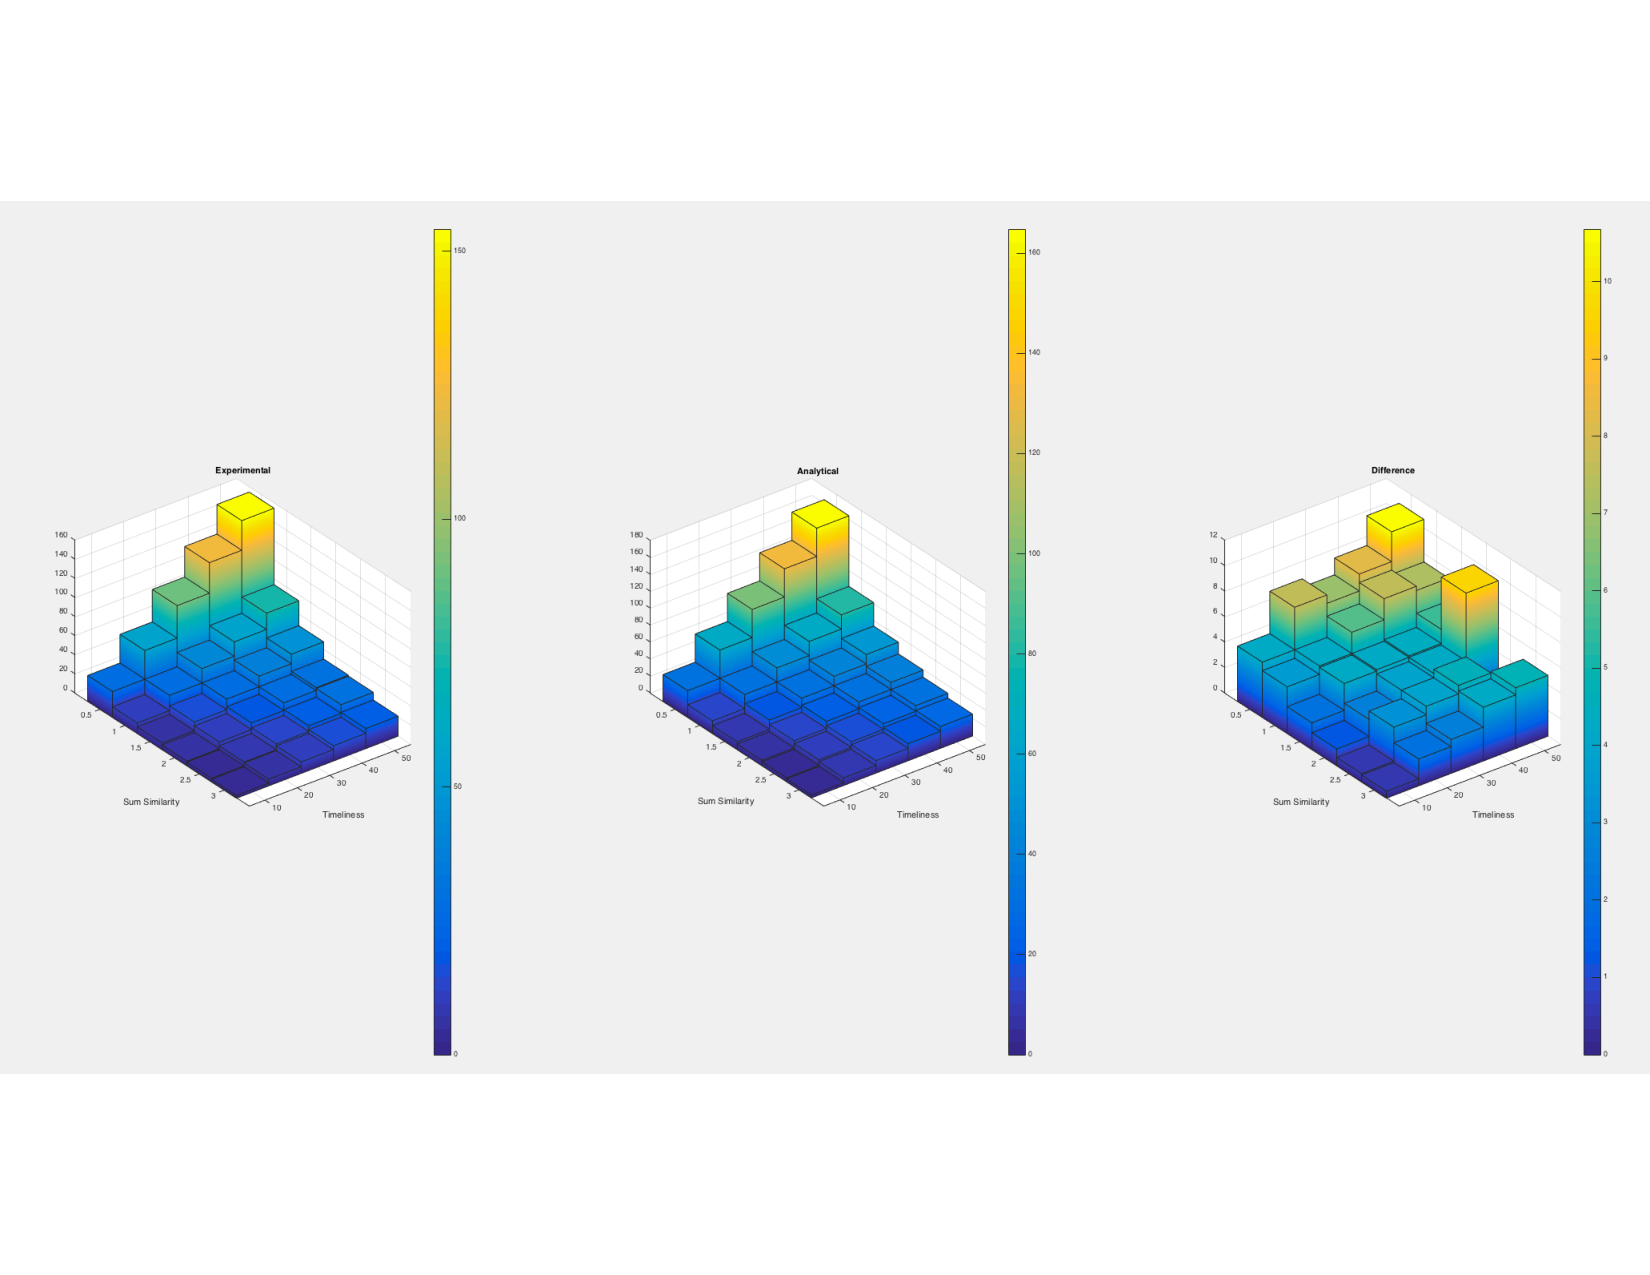
\includegraphics[scale=0.65]{result_expl_figs/line_unicast_large_buffers.pdf}
    \caption{Line Network - No Multihop Consideration - [Experimental, Analytical, Difference(Num packets)]}
    \label{fig:line_net_uni_no_mhop}
\end{figure*}

When I include the multi hop consideration in this scenario, the analytical results I get are significantly different.  This is shown in Figure \ref{fig:line_net_uni_mhop} with the difference showing the absolute value.  Here, we actually miss by much more.

\begin{figure*}
    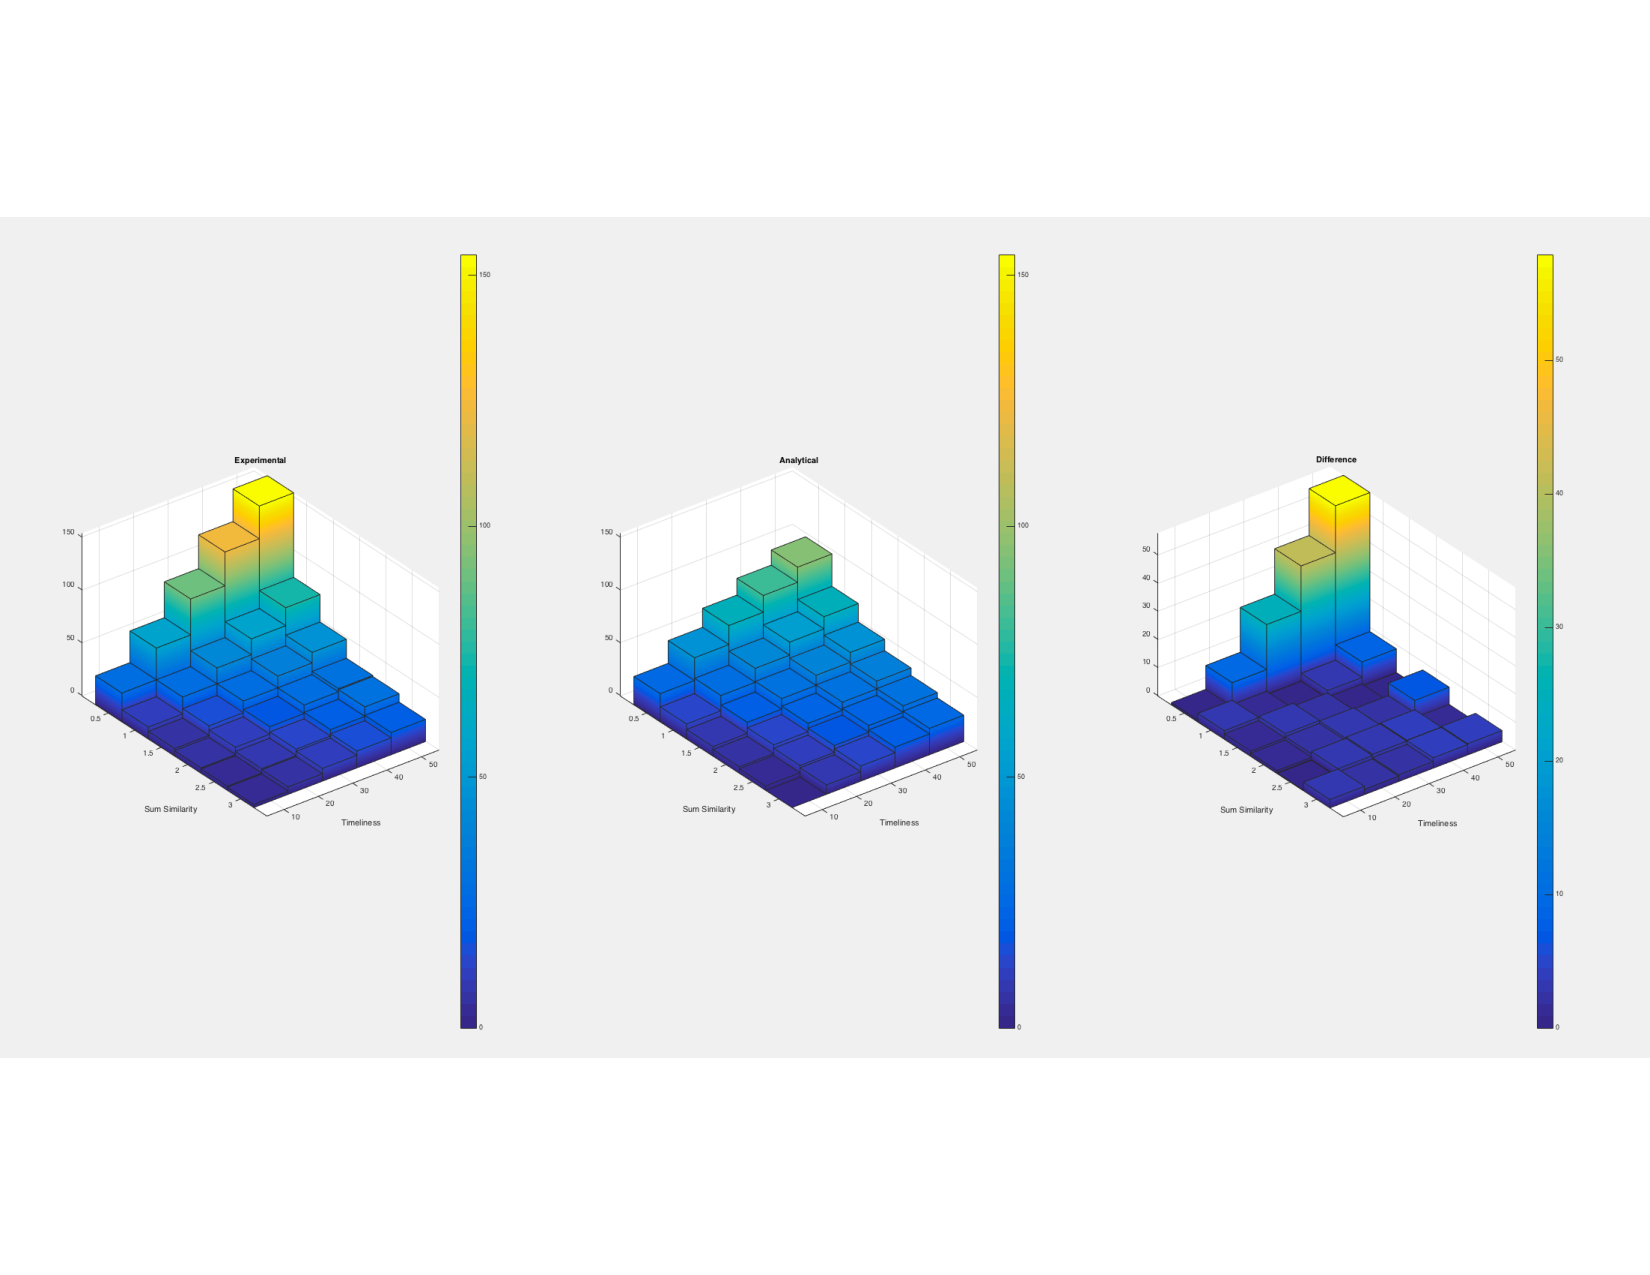
\includegraphics[scale=0.65]{result_expl_figs/line_unicast_IS_50_CR_2_mhop.pdf}
    \caption{Line Network - Including Multihop Consideration - [Experimental, Analytical, Difference(Num packets)]}
    \label{fig:line_net_uni_mhop}
\end{figure*}

\subsection{Grid Network}
Now, here's where things get a little tricky.  The initial results that do not include any multi hop consideration are off by around $150$ packets at the worst, which turns out to be around $30\%$.  These results are in Figure \ref{fig:grid_net_uni_no_mhop}.
\begin{figure*}
    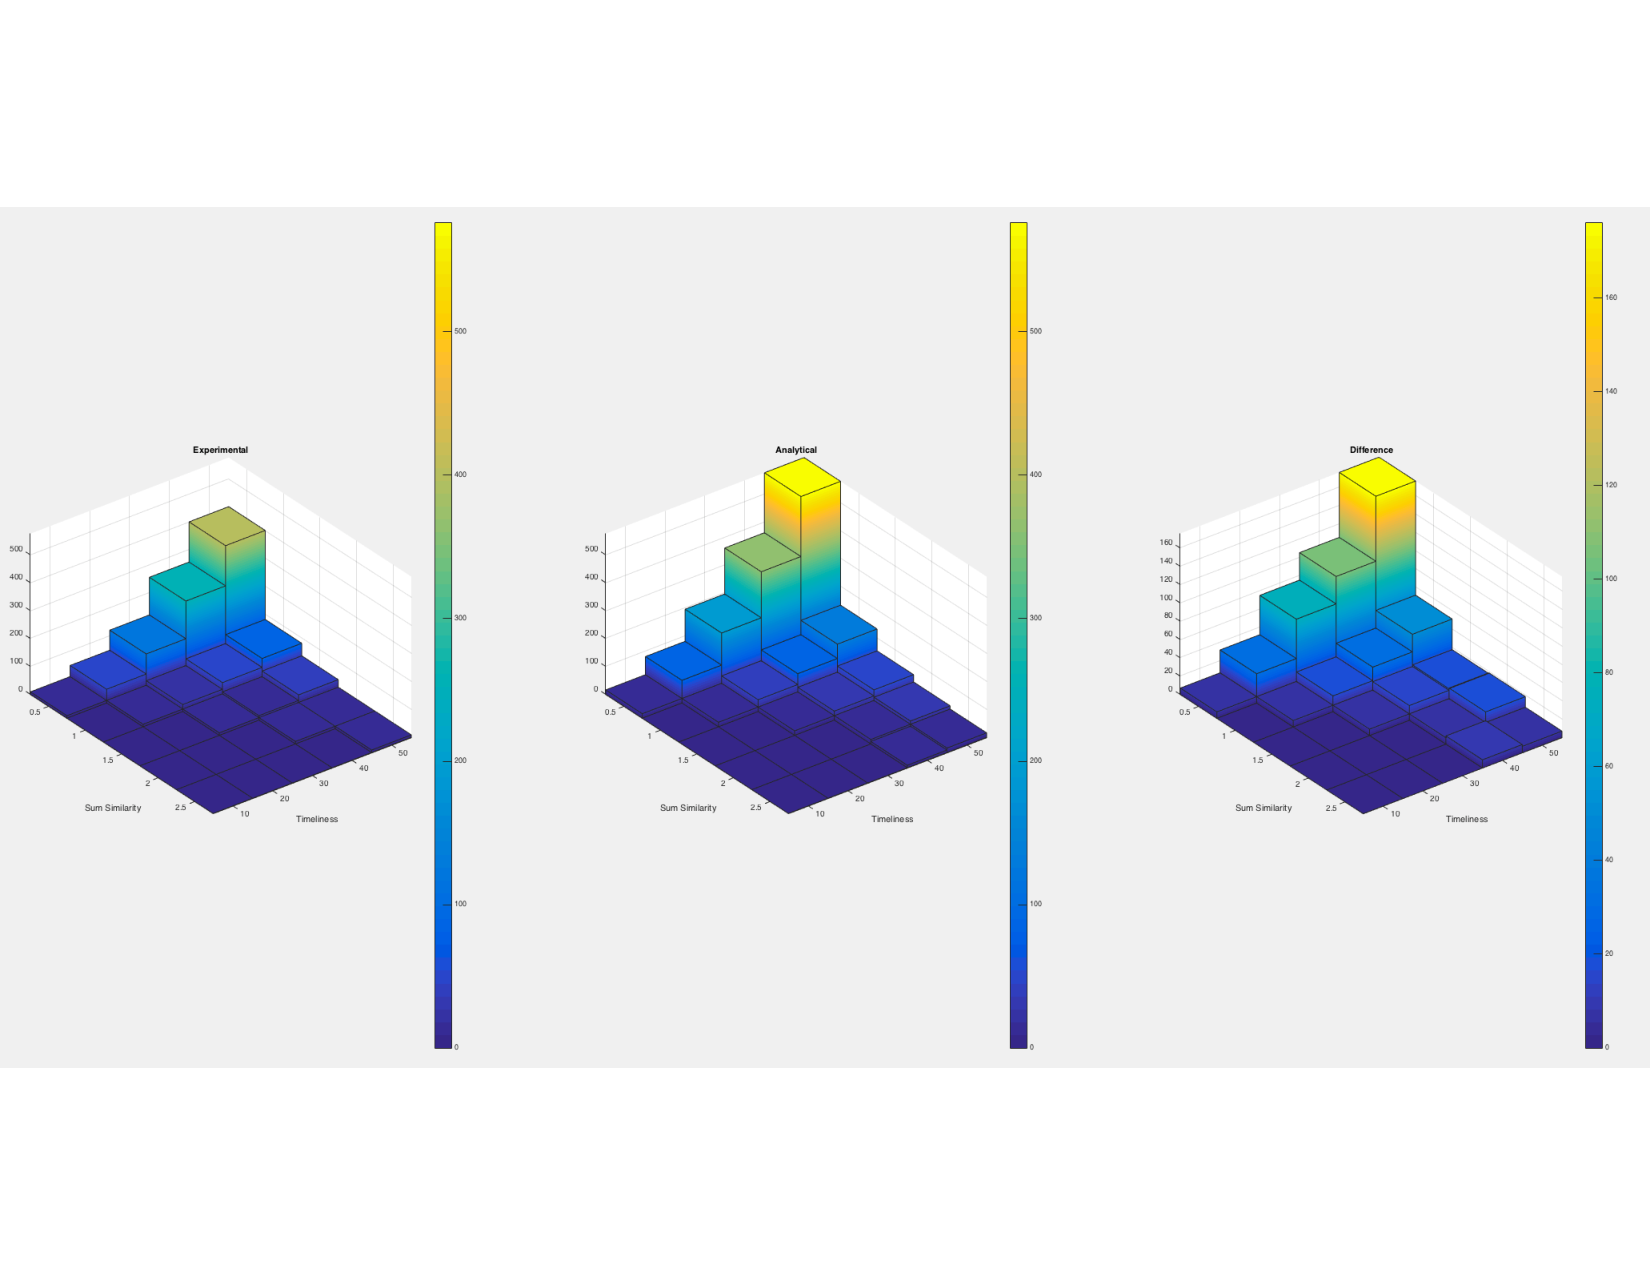
\includegraphics[scale=0.65]{result_expl_figs/grid_IS_100_CR_2.pdf}
    \caption{Grid Network - No Multihop Consideration - [Experimental, Analytical, Difference(Num packets)]}
    \label{fig:grid_net_uni_no_mhop}
\end{figure*}

When I include the multi hop consideration in this scenario from the equation above, which simply uses the average path length over the entire network, the results actually improve to become quite close.  Here, I switched to a percentage difference in the right-most figure because it was the easiest to see in this case.  This set of results is in Figure \ref{fig:grid_net_uni_mhop}.  You can't see actual numbers here, but the worst is around 30\% for some of the trials, which is actually also an absolute difference of about 30 nodes at the maximum.  The largest scalability values are the closest here, though.  At Sum Sim = $0.5$ and a timeliness of $50$, the results are almost a perfect match.

\begin{figure*}
    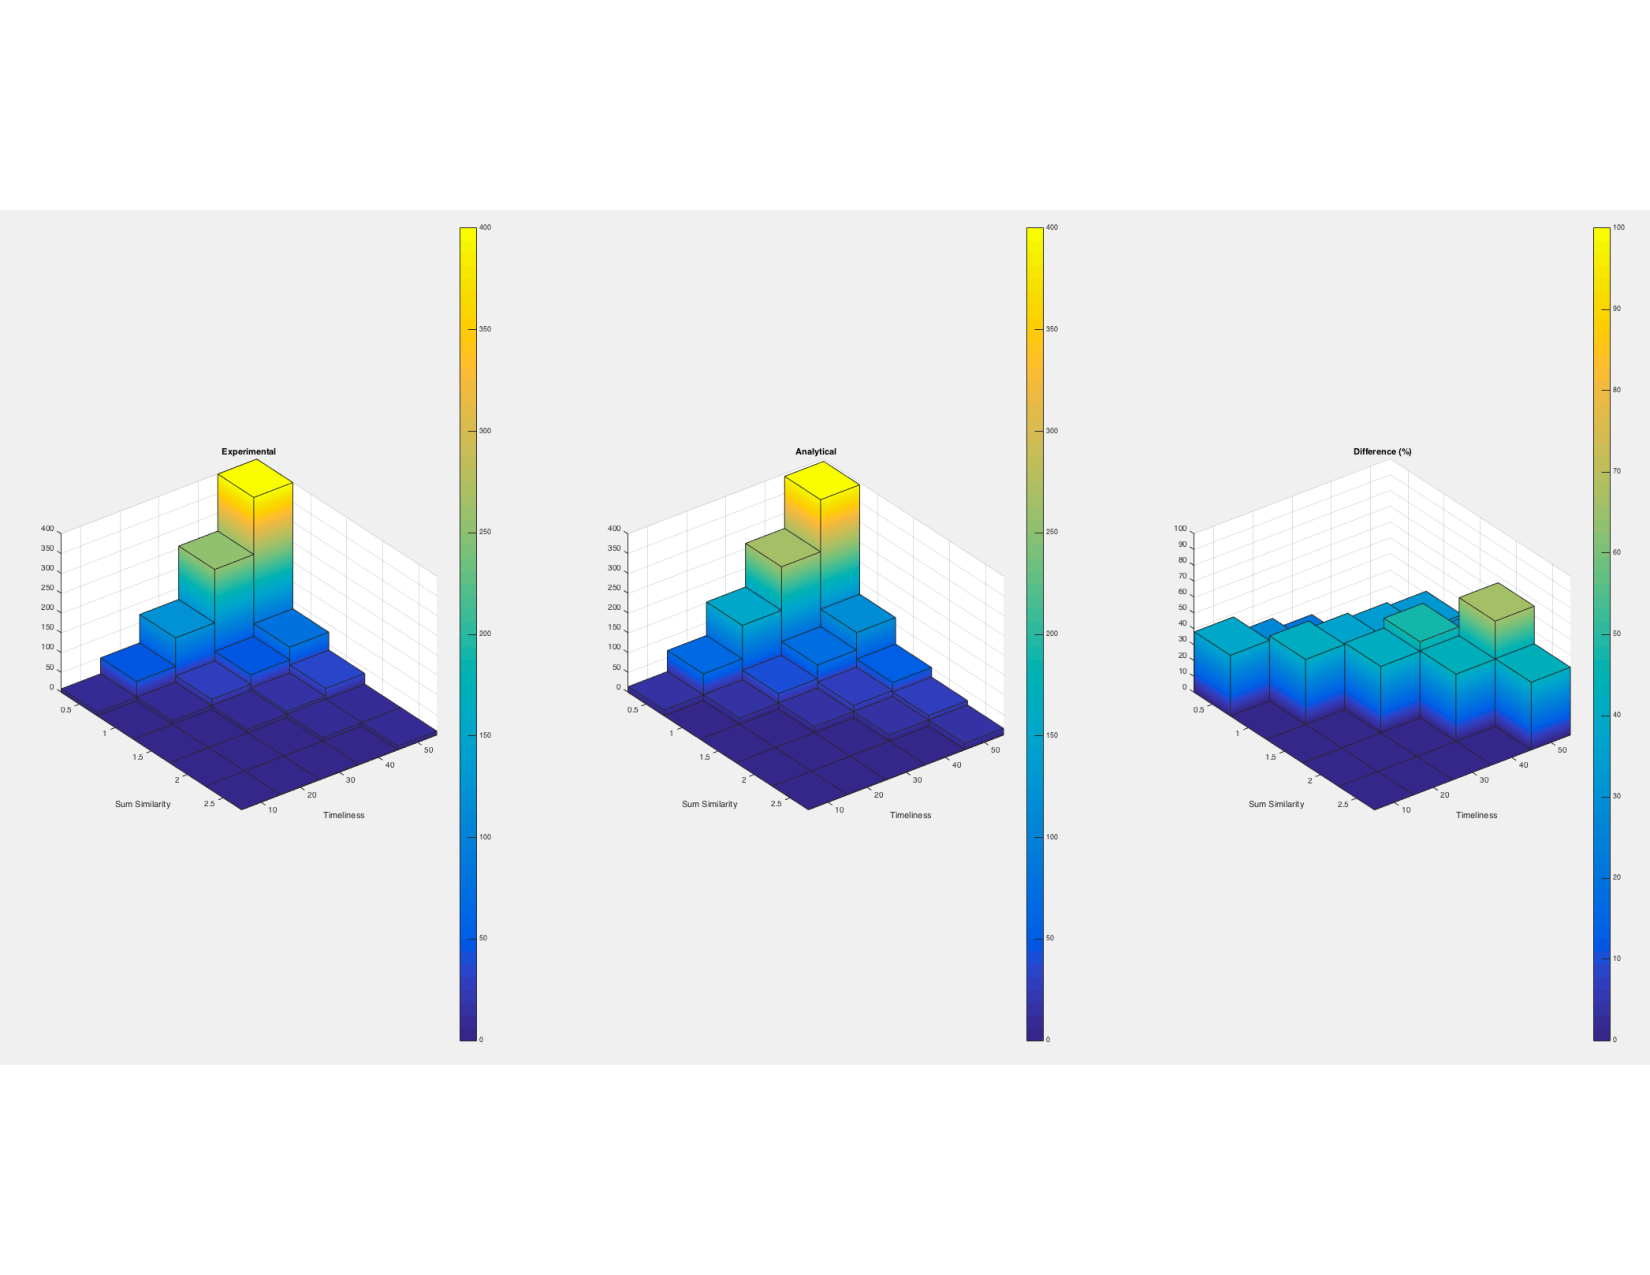
\includegraphics[scale=0.65]{result_expl_figs/grid_IS_100_CR_2_mhop.pdf}
    \caption{Grid Network - Including Multihop Consideration - [Experimental, Analytical, Difference(\%)]}
    \label{fig:grid_net_uni_mhop}
\end{figure*}

%\appendix
%\input{sections/random_explanation}
% conference papers do not normally have an appendix


% use section* for acknowledgement
%\section*{Acknowledgment}


%The authors would like to thank...


% trigger a \newpage just before the given reference
% number - used to balance the columns on the last page
% adjust value as needed - may need to be readjusted if
% the document is modified later
%\IEEEtriggeratref{8}
% The "triggered" command can be changed if desired:
%\IEEEtriggercmd{\enlargethispage{-5in}}

% references section

% can use a bibliography generated by BibTeX as a .bbl file
% BibTeX documentation can be easily obtained at:
% http://www.ctan.org/tex-archive/biblio/bibtex/contrib/doc/
% The IEEEtran BibTeX style support page is at:
% http://www.michaelshell.org/tex/ieeetran/bibtex/
%\bibliographystyle{IEEEtran}
% argument is your BibTeX string definitions and bibliography database(s)
%\bibliography{IEEEabrv,../bib/paper}
%
% <OR> manually copy in the resultant .bbl file
% set second argument of \begin to the number of references
% (used to reserve space for the reference number labels box)
%\begin{thebibliography}{1}


\bibliographystyle{unsrt}

\bibliography{references}

%\bibitem{IEEEhowto:kopka}
%H.~Kopka and P.~W. Daly, \emph{A Guide to \LaTeX}, 3rd~ed.\hskip 1em plus
%  0.5em minus 0.4em\relax Harlow, England: Addison-Wesley, 1999.

%\end{thebibliography}




% that's all folks
\end{document}


